\subsection{Проектирование алгоритма работы программы}
\label{sec:design:algorithm}

На рисунке~\ref{sec:design:main_algorithm_scheme} представлена схема алгоритма работы программного средства создания веб-приложений с помощью готовых графических компонентов. 
На ней отражены такие возможные действия, доступные для выполнения, как применение пресетов и компонентов, редактирование свойств компонентов, удаление компонентов. 

\begin{figure}[ht]
\centering
    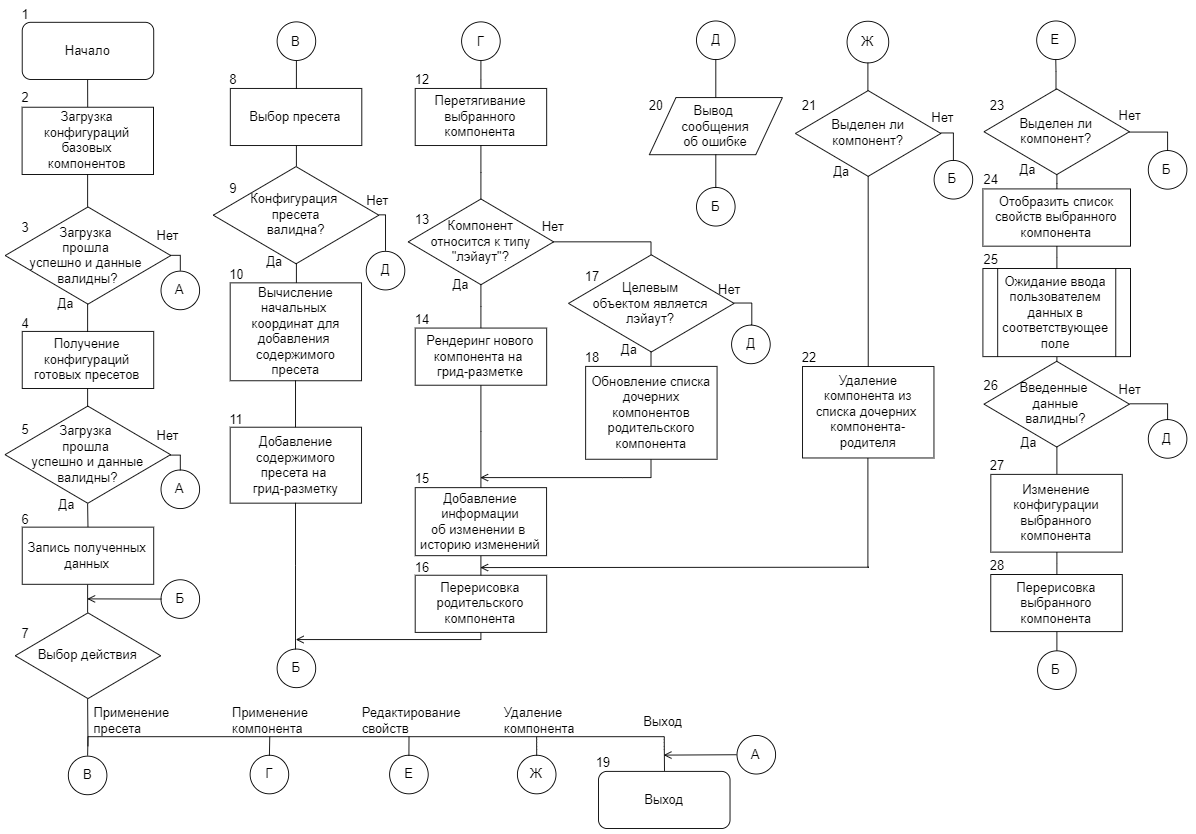
\includegraphics[scale=0.40]{schema_main.png}
    \caption{Диаграмма прецедентов приложения}
    \label{sec:design:main_algorithm_scheme}
\end{figure}
    
В зависимости от конкретного действия, каждое содержит в себе собственные шаги реализации. 
Так при выборе действия <<Применение компонента>> происходит отрисовка одного компонента, перетянутого пользователем на грид-разметку, а при выборе <<Применение пресета>> происходит отрисовка целой совокупности компонентов. <<Редактирование свойств>> содержит в себе проверку введённых данных на корректность и процесс измненения свойств выбранного компонента. <<Удаление компонента>> осуществляется при выбора компонента и нажатии кнопки удаления, в таком случае все дочерние элементы (если они есть) также удаляются, после чего родительский компонент (если выбранный удаляемый компонент не был помещен непосредственно на грид-разметку) также перерисовывается. Каждое добавление компонента влечет за собой дополнительное действие в виде запоминания выполненного действия в истории изменений, чтобы в случае необходимости <<откатить>> последнее добавление элемента.

